%----------------------------------------------------------------------------------------
%	PACKAGES AND DOCUMENT CONFIGURATIONS
%----------------------------------------------------------------------------------------

\documentclass{article}


\usepackage{graphicx} % Required for the inclusion of images
\usepackage{subfigure} % Required for the inclusion of images
\usepackage{natbib} % Required to change bibliography style to APA
\usepackage{amsmath} % Required for some math elements 
\usepackage{graphicx}
\usepackage{listings} % 插入代码块
\usepackage{pythonhighlight}
\usepackage{color}

\lstset{ %
	basicstyle=\linespread{1.0}\footnotesize\ttfamily,       % the size of the fonts that are used for the code
	numbers=left,                   % where to put the line-numbers
	numberstyle=\footnotesize\ttfamily,      % the size of the fonts that are used for the line-numbers
	stepnumber=1,                   % the step between two line-numbers. If it is 1 each line will be numbered
	numbersep=5pt,                  % how far the line-numbers are from the code
	backgroundcolor=\color{white},  % choose the background color. You must add \usepackage{color}
	showspaces=false,               % show spaces adding particular underscores
	showstringspaces=false,         % underline spaces within strings
	showtabs=false,                 % show tabs within strings adding particular underscores
	frame=lines,
	tabsize=2,          % sets default tabsize to 2 spaces
	captionpos=b,           % sets the caption-position to bottom
	breaklines=true,        % sets automatic line breaking
	breakatwhitespace=false,    % sets if automatic breaks should only happen at whitespace
	escapeinside={\%*}{*)},          % if you want to add a comment within your code
	float,
	aboveskip=15pt,
	morekeywords = {mrmovl, rmmovl, rrmovl, andl, xorl, iaddl, jle, jl, je, jg, jmp},
	keywordstyle=\bfseries\color{blue},
	commentstyle=\itshape\color{purple!40!black},
	identifierstyle=\color{black},
	stringstyle=\color{orange},
}


%\usepackage{times} % Uncomment to use the Times New Roman font

%----------------------------------------------------------------------------------------
%	DOCUMENT INFORMATION
%----------------------------------------------------------------------------------------

\title{\textbf{Project 1: Optimizing the Performance of a Pipelined Processor}} % Title

\author{Li Zikun, 521120910252, lizk1024@sjtu.edu.cn \\
        Hu Chenzhi, 521021910107,  ether-wind@sjtu.edu.cn \\
        Wang Shunyu, 521120910244, lzywsy03@sjtu.edu.cn } % Author name and email

\date{\today} % Date for the report

\begin{document}

\maketitle % Insert the title, author and date

\section{Introduction}

In this project, we have three parts. In part A, we wrote some simple Y86 programs, for example, sum, rsum and copy , to get familiar with the usage of Y86. In part B, we made a little modification to the SEQ processor for a new instruction: \verb |iaddl|. In part C, which is the critical and the hardest part of the whole lab, we optimized the performance of the pipelined processor with the ncopy function.\\

\noindent[Li and Wang finished part A and B together, Hu finished part C, and the three of us finished the report together.]

\section{Experiments}

\subsection{Part A}

\subsubsection{Analysis}

In part A, we were tasked with using \verb |Y86 ISA| to implement \verb |C| language code functionality. Our objective was to use Y86 assembly language to achieve the same functionality as the code in \verb |example.c|, and we accomplished two tasks: 1) traverse a linked list and return the sum of all long-type integers in the list (using both iterative and recursive algorithms), and 2) copy a sequence of long-type integers to another memory address. 

To achieve this, we first studied Y86 register names, instruction format, and execution method. The core techniques for each of the three different functionalities are as follows:

1. For the \verb |sum| function, we traversed the linked list using a loop to sum all \verb |long-type| integers. We did this by loading and storing memory data, iterating through each element of the list, and incrementally summing the values of the long integers in the list with the help of registers. We used the \verb |\%eax| register to record current element value, \verb |\%edx| register to record the address of next element, and \verb |\%ecx| register to record the sum of all elements. If there are more elements after the current one, we jump back to the loop to continue processing. If the end of the linked list is reached, the program returns the sum stored in the \verb |\%ecx| register. A stack is also used to ensure proper program execution.

2. For the \verb |\%rsum| function, we used recursion to sum \verb |long-type| integers in a linked list. We loaded and stored memory data in the same way as in the "sum" function, but instead of a loop, we relied on recursive calls to the \verb |rsum_list| function to process each element in the list. Each time an element is processed, its value is added to the \verb |\%eax| register, and the address of the next element and the current element's value are stored in the \verb |\%edx| and\verb |\%edi| registers respectively. If \verb |\%edx| is equal to zero, the recursion ends, and the result stored in the \verb |\%eax| register is returned. A stack is also used to ensure proper program execution.

3. For the \verb |copy_block| function, the code copies the data from a source address \verb |src| to a destination address \verb |dest| by looping through the data in the source address and copying it to the corresponding location in the destination address. The main function in the code calls the \verb |copy_block| function to perform the data copy. A stack is used to store the original information saved in registers before function invocation by using the \verb |pushl|, and is restored using the \verb |popl| instruction at the end of the function execution.

The challenges in implementing these functionalities included understanding how many registers we could use in our code, learning various \verb |Y86 ISA| opcodes and instruction formats, as well as understanding and using registers to store and control data flow, controlling program flow by using various jump instructions, mastering stack operations, and writing complex algorithms to traverse a linked list and copy a block of memory. It was also important to have proficient debugging and error fixing skills.

\subsubsection{Code}

The core code for three tasks in Part A is respectively in Code Listing \ref{cd:sum}, \ref{cd:rsum}, \ref{cd:copy}.

\begin{lstlisting}[caption={Core Code of sum.ys}, label={cd:sum}]
.align 4				# Sample linked list
ele1:				# Define memory with label ele1
        .long 0x00a
        .long ele2
ele2:				# Define memory with label ele2
        .long 0x0b0
        .long ele3
ele3:				# Define memory with label ele3
        .long 0xc00
        .long 0

main:	
	irmovl ele1,%edx		# Initialize %edx with the address of ele1 	
        call sum_list			# Call the sum_list function
	ret

sum_list:				# sums a list of long integers starting at the address in %edx
	irmovl $0,%ecx		# Set the initial value of %ecx to 0
	
loop:	mrmovl (%edx),%eax	# Load memory address at %edx into %eax 
        addl %eax,%ecx		# Add to %ecx
        mrmovl 4(%edx ),%eax		# Load the next memory address to %eax
        rrmovl %eax,%edx		# Move the next address to %edx 
        
test:   andl %edx,%edx		# Check if %edx is equal to 0
        jne loop			# If not 0 jump back to loop
        ret				# Return the sum stored in %ecx
\end{lstlisting}
\begin{lstlisting}[caption={Core Code of rsum.ys}, label={cd:rsum}]
.align 4				# Sample linked list
ele1:				# Define memory with label ele1
        .long 0x00a
        .long ele2
ele2:				# Define memory with label ele2
        .long 0x0b0
        .long ele3
ele3:				# Define memory with label ele3
        .long 0xc00
        .long 0

main:
	irmovl ele1,%edx		# Initialize %edx with the address of ele1 	
        call rsum_list			# Calls the sum_list function
	ret
rsum_list:
	pushl %edi		# Push %edi into stack
	irmovl $0,%eax		# Set the initial value of result register %eax to 0
	andl %edx,%edx		# Check if %edx is equal to 0
	je re			# If 0 jump to re
	mrmovl (%edx),%edi	# Load memory address at %edx into %edi 
	mrmovl 4(%edx),%edx	# Load next memory address of %edx into %edx
	call rsum_list		# Call the rsum_list function
	addl %edi,%eax		# Add value of %edi to %eax
re:
	popl %edi		# Pop %edi out of stack
	ret			# Return the sum stored in %eax
\end{lstlisting}
\begin{lstlisting}[caption={Core Code of copy.ys}, label={cd:copy}]
.align 4 
src: 				# Source block 
	.long 0x00a 
	.long 0x0b0 
	.long 0xc00 

dest: 				# Destination block 
	.long 0x111 
	.long 0x222 
	.long 0x333 

main: 
	irmovl src, %esi 	# Initialize source address 
	irmovl dest, %edi 	# Initialize destination address 
	irmovl $3, %edx 	# Initialize count 
	call copy_block 	# Call copy_block to perform the copy 
	ret 
	
copy_block: 
	pushl %ebp 		# Save old frame pointer 
	pushl %ebx 		# Save callee-saved register 
	pushl %ecx 		# Save callee-saved register 
	xorl %eax, %eax 	# Initialize accumulator 
	irmovl $4, %ecx 	# Set increment value for addresses 
	irmovl $1, %ebx 	# Set decrement value for count 

loop: 
	andl %edx, %edx 	# Check if count is greater than zero 
	jle finish # If not, jump to finish 
	mrmovl (%esi), %ebp	# Move data from source address to temporary register 
	rmmovl %ebp, (%edi) 	# Move data from temporary register to destination address 
	xorl %ebp, %eax 	# Accumulate negated data value 
	addl %ecx, %esi 	# Update source address 
	addl %ecx, %edi 	# Update destination address 
	subl %ebx, %edx 	# Decrement count 
	jmp loop 		# Jump to loop 
	
finish: 
	popl %ecx 		# Restore callee-saved register 
	popl %ebx 		# Restore callee-saved register 
	popl %ebp 		# Restore old frame pointer 
	ret 			# Return to the caller 
\end{lstlisting}

\subsubsection{Evaluation}


We have written three functions based on the original C code, and after consulting the material in the book, we have produced Y86 versions of them. After examination, as the result shown in Figure \ref{fig:sum}, \ref{fig:rsum}, \ref{fig:copy}, all three functions are correct.

\begin{figure}[htbp]
\centering
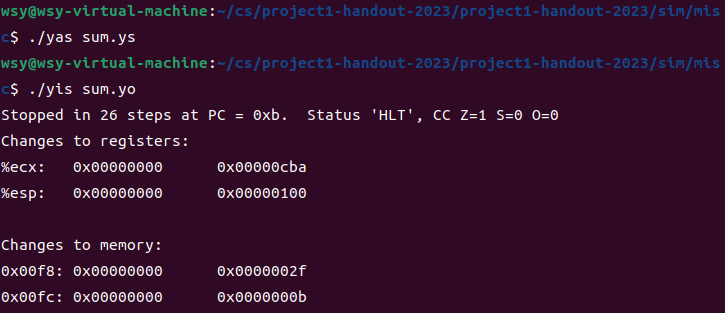
\includegraphics[width=0.7\textwidth]{figure/ptasum.png}
\caption{Result of sum.ys} %最终文档中希望显示的图片标题
\label{fig:sum} %用于文内引用的标签
\end{figure}

\begin{figure}[htbp]
\centering
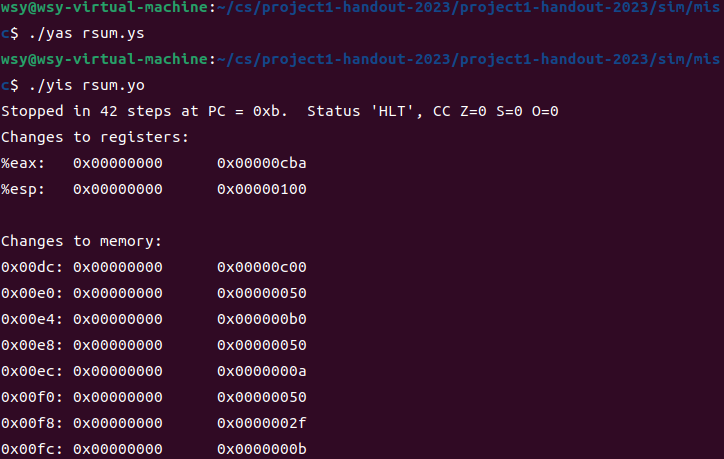
\includegraphics[width=0.7\textwidth]{figure/ptaysum.png}
\caption{Result of rsum.ys} %最终文档中希望显示的图片标题
\label{fig:rsum} %用于文内引用的标签
\end{figure}

\begin{figure}[htbp]
\centering
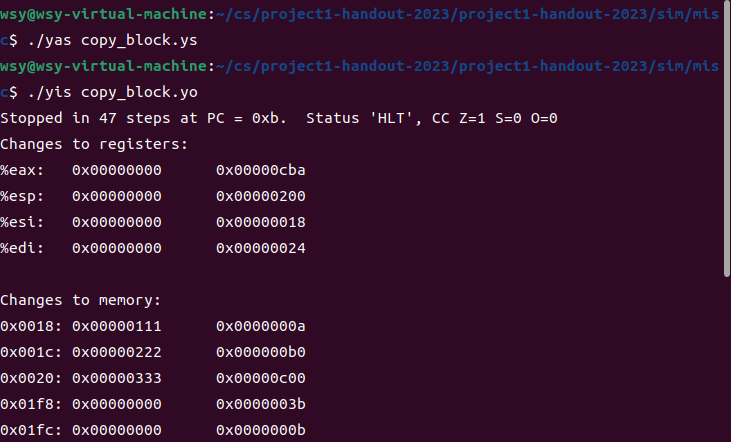
\includegraphics[width=0.7\textwidth]{figure/ptacblock.png}
\caption{Result of copy.ys} %最终文档中希望显示的图片标题
\label{fig:copy} %用于文内引用的标签
\end{figure} 

\subsection{Part B}

\subsubsection{Analysis}

In this part, we are going to extend the SEQ processor for a new instruction: \verb |iaddl|, whose function is to add an immediate operand to a register. We will modify the file \verb |seq-full.hcl| to enable the instruction \verb|iaddl|. We will dig into the execution of the instruction, and figure out the details in each stage of the instruction. First, we append the new instruction to the Fetch stage. Then we append it to the bool \verb |need_regids| and \verb |need_valC|, because it needs to read the register B and the immediate operand. In the Decode stage we set the \verb |srcB| to \verb |rB| and \verb |dstE| to \verb |rB| to store the result. In the memory stage, we set the \verb |aluA| to \verb |valC| and \verb |aluB| to \verb |valB| and append it to the \verb |setCC| because CC needs to be updated.

\subsubsection{Code}

The code of \verb|seq-full.hcl| is shown in Code Listing \ref{cd:seq}.

\begin{lstlisting}[caption={seq-full.hcl}, label={cd:seq}]
#/* $begin seq-all-hcl */
####################################################################
#  HCL Description of Control for Single Cycle Y86 Processor SEQ   #
#  Copyright (C) Randal E. Bryant, David R. O'Hallaron, 2010       #
####################################################################

## Your task is to implement the iaddl instruction
## The file contains a declaration of the icodes
## for iaddl (IIADDL) .
## Your job is to add the rest of the logic to make it work

####################################################################
#    C Include's.  Don't alter these                               #
####################################################################

quote '#include <stdio.h>'
quote '#include "isa.h"'
quote '#include "sim.h"'
quote 'int sim_main(int argc, char *argv[]);'
quote 'int gen_pc(){return 0;}'
quote 'int main(int argc, char *argv[])'
quote '  {plusmode=0;return sim_main(argc,argv);}'

####################################################################
#    Declarations.  Do not change/remove/delete any of these       #
####################################################################

##### Symbolic representation of Y86 Instruction Codes #############
intsig INOP 	'I_NOP'
intsig IHALT	'I_HALT'
intsig IRRMOVL	'I_RRMOVL'
intsig IIRMOVL	'I_IRMOVL'
intsig IRMMOVL	'I_RMMOVL'
intsig IMRMOVL	'I_MRMOVL'
intsig IOPL	'I_ALU'
intsig IJXX	'I_JMP'
intsig ICALL	'I_CALL'
intsig IRET	'I_RET'
intsig IPUSHL	'I_PUSHL'
intsig IPOPL	'I_POPL'
# Instruction code for iaddl instruction
intsig IIADDL	'I_IADDL'

##### Symbolic represenations of Y86 function codes                  #####
intsig FNONE    'F_NONE'        # Default function code

##### Symbolic representation of Y86 Registers referenced explicitly #####
intsig RESP     'REG_ESP'    	# Stack Pointer
intsig REBP     'REG_EBP'    	# Frame Pointer
intsig RNONE    'REG_NONE'   	# Special value indicating "no register"

##### ALU Functions referenced explicitly                            #####
intsig ALUADD	'A_ADD'		# ALU should add its arguments

##### Possible instruction status values                             #####
intsig SAOK	'STAT_AOK'		# Normal execution
intsig SADR	'STAT_ADR'	# Invalid memory address
intsig SINS	'STAT_INS'	# Invalid instruction
intsig SHLT	'STAT_HLT'	# Halt instruction encountered

##### Signals that can be referenced by control logic ####################

##### Fetch stage inputs		#####
intsig pc 'pc'				# Program counter
##### Fetch stage computations		#####
intsig imem_icode 'imem_icode'		# icode field from instruction memory
intsig imem_ifun  'imem_ifun' 		# ifun field from instruction memory
intsig icode	  'icode'		# Instruction control code
intsig ifun	  'ifun'		# Instruction function
intsig rA	  'ra'			# rA field from instruction
intsig rB	  'rb'			# rB field from instruction
intsig valC	  'valc'		# Constant from instruction
intsig valP	  'valp'		# Address of following instruction
boolsig imem_error 'imem_error'		# Error signal from instruction memory
boolsig instr_valid 'instr_valid'	# Is fetched instruction valid?

##### Decode stage computations		#####
intsig valA	'vala'			# Value from register A port
intsig valB	'valb'			# Value from register B port

##### Execute stage computations	#####
intsig valE	'vale'			# Value computed by ALU
boolsig Cnd	'cond'			# Branch test

##### Memory stage computations		#####
intsig valM	'valm'			# Value read from memory
boolsig dmem_error 'dmem_error'		# Error signal from data memory


####################################################################
#    Control Signal Definitions.                                   #
####################################################################

################ Fetch Stage     ###################################

# Determine instruction code
int icode = [
        imem_error: INOP;
        1: imem_icode;		# Default: get from instruction memory
];

# Determine instruction function
int ifun = [
        imem_error: FNONE;
        1: imem_ifun;		# Default: get from instruction memory
];

bool instr_valid = icode in 
        { INOP, IHALT, IRRMOVL, IIRMOVL, IRMMOVL, IMRMOVL,
                IOPL, IJXX, ICALL, IRET, IPUSHL, IPOPL, IIADDL };

# Does fetched instruction require a regid byte?
bool need_regids =
        icode in { IRRMOVL, IOPL, IPUSHL, IPOPL, 
                        IIRMOVL, IRMMOVL, IMRMOVL, IIADDL };

# Does fetched instruction require a constant word?
bool need_valC =
        icode in { IIRMOVL, IRMMOVL, IMRMOVL, IJXX, ICALL, IIADDL};

################ Decode Stage    ###################################

## What register should be used as the A source?
int srcA = [
        icode in { IRRMOVL, IRMMOVL, IOPL, IPUSHL  } : rA;
        icode in { IPOPL, IRET } : RESP;
        1 : RNONE; # Don't need register
];

## What register should be used as the B source?
int srcB = [
        icode in { IOPL, IRMMOVL, IMRMOVL, IIADDL } : rB;
        icode in { IPUSHL, IPOPL, ICALL, IRET } : RESP;
        1 : RNONE;  # Don't need register
];

## What register should be used as the E destination?
int dstE = [
        icode in { IRRMOVL } && Cnd : rB;
        icode in { IIRMOVL, IOPL, IIADDL } : rB;
        icode in { IPUSHL, IPOPL, ICALL, IRET } : RESP;
        1 : RNONE;  # Don't write any register
];

## What register should be used as the M destination?
int dstM = [
        icode in { IMRMOVL, IPOPL } : rA;
        1 : RNONE;  # Don't write any register
];

################ Execute Stage   ###################################

## Select input A to ALU
int aluA = [
        icode in { IRRMOVL, IOPL } : valA;
        icode in { IIRMOVL, IRMMOVL, IMRMOVL, IIADDL } : valC;
        icode in { ICALL, IPUSHL } : -4;
        icode in { IRET, IPOPL } : 4;
        # Other instructions don't need ALU
];

## Select input B to ALU
int aluB = [
        icode in { IRMMOVL, IMRMOVL, IOPL, ICALL, 
                        IPUSHL, IRET, IPOPL, IIADDL} : valB;
        icode in { IRRMOVL, IIRMOVL } : 0;
        # Other instructions don't need ALU
];

## Set the ALU function
int alufun = [
        icode == IOPL : ifun;
        1 : ALUADD;
];

## Should the condition codes be updated?
bool set_cc = icode in { IOPL, IIADDL };

################ Memory Stage    ###################################

## Set read control signal
bool mem_read = icode in { IMRMOVL, IPOPL, IRET };

## Set write control signal
bool mem_write = icode in { IRMMOVL, IPUSHL, ICALL };

## Select memory address
int mem_addr = [
        icode in { IRMMOVL, IPUSHL, ICALL, IMRMOVL } : valE;
        icode in { IPOPL, IRET } : valA;
        # Other instructions don't need address
];

## Select memory input data
int mem_data = [
        # Value from register
        icode in { IRMMOVL, IPUSHL } : valA;
        # Return PC
        icode == ICALL : valP;
        # Default: Don't write anything
];

## Determine instruction status
int Stat = [
        imem_error || dmem_error : SADR;
        !instr_valid: SINS;
        icode == IHALT : SHLT;
        1 : SAOK;
];

################ Program Counter Update ############################

## What address should instruction be fetched at

int new_pc = [
        # Call.  Use instruction constant
        icode == ICALL : valC;
        # Taken branch.  Use instruction constant
        icode == IJXX && Cnd : valC;
        # Completion of RET instruction.  Use value from stack
        icode == IRET : valM;
        # Default: Use incremented PC
        1 : valP;
];
#/* $end seq-all-hcl */
\end{lstlisting}

\subsubsection{Evaluation}
\begin{figure}[htbp]
\centering
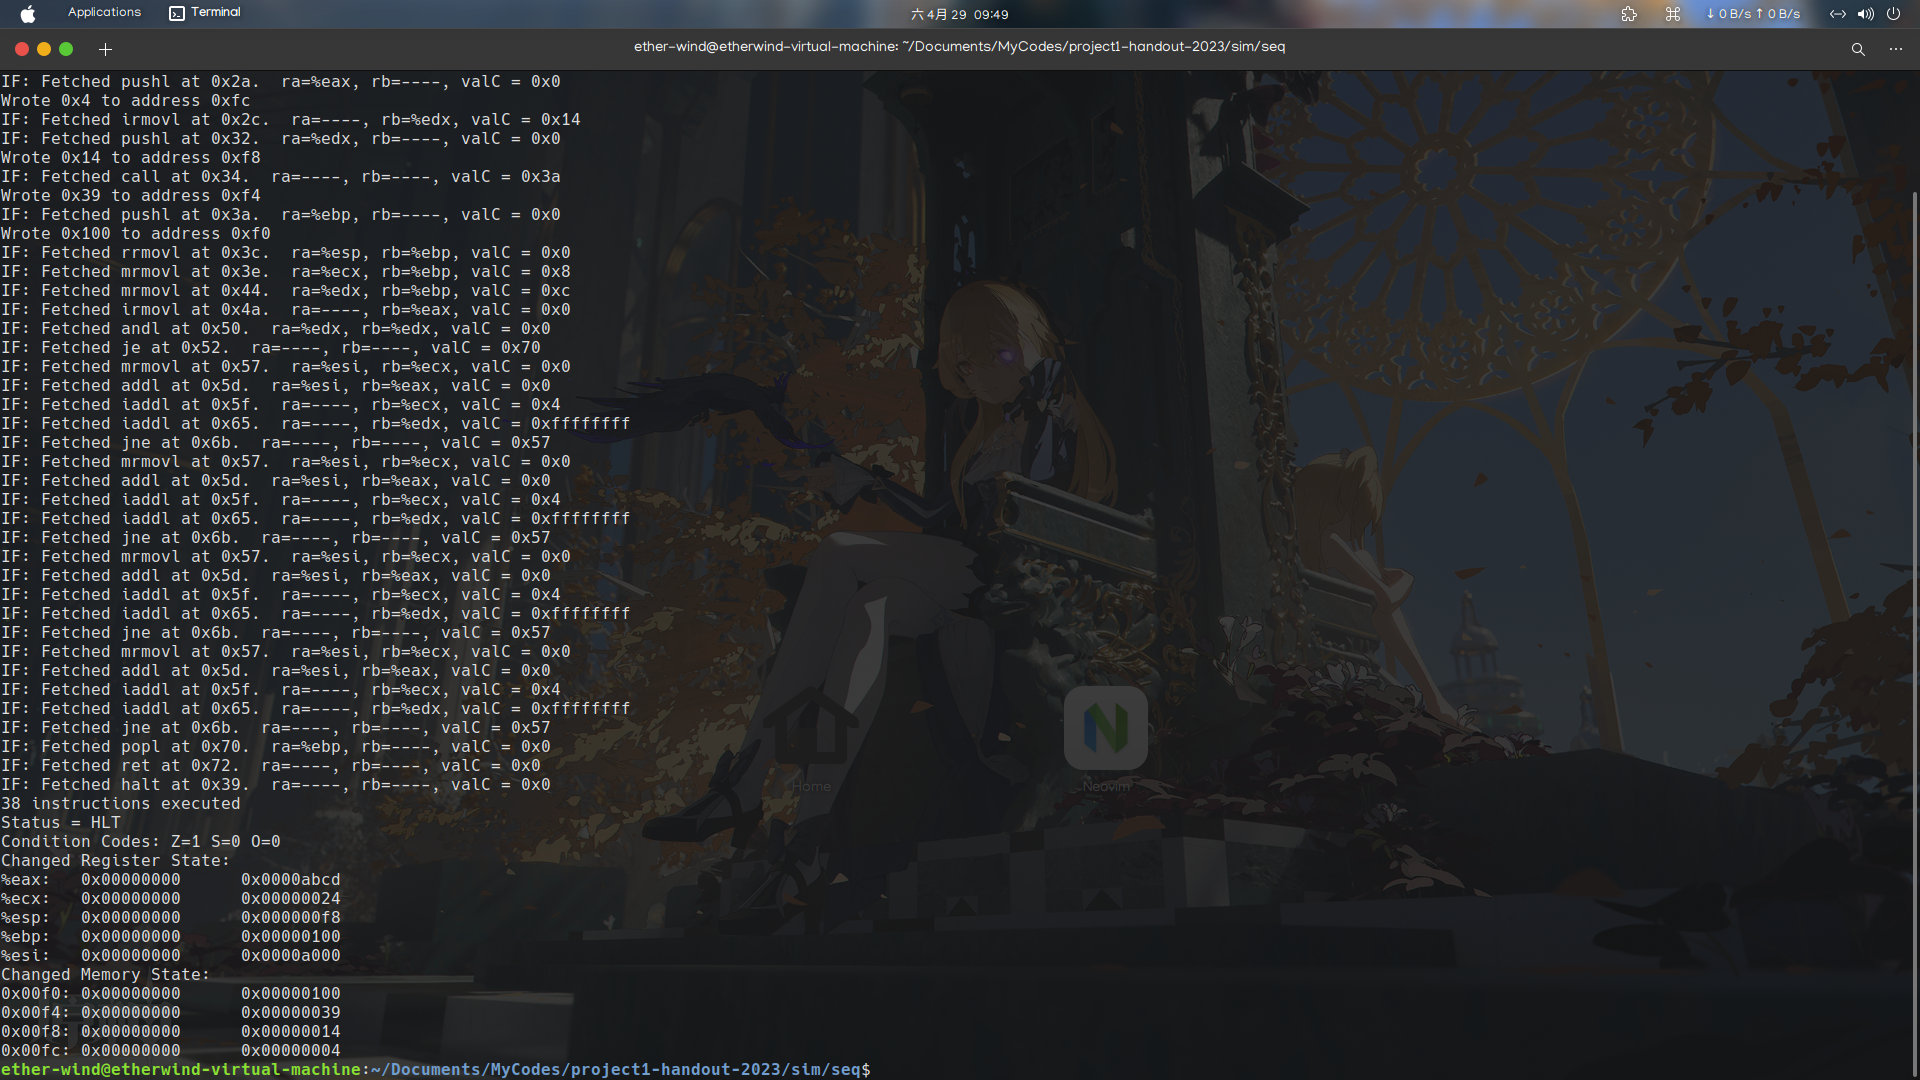
\includegraphics[width=1\textwidth]{figure/ptb.png}
\caption{Result of Part B}
\label{fig:seq}
\end{figure} 

We made extension to the file \verb |seq-full.hcl| to enable the instruction \verb |iaddl|, and then formed \verb |ssim| to test it. As the result shown in Figure \ref{fig:seq}, we have the correct result

\subsection{Part C}

\subsubsection{Analysis}

Part C can be devided into two parts: the first part is addding \verb|iaddl| operation to the pipeline, which is the same as Part B. The second part is optimizing the performance of \verb|ncopy.ys|.

To optimize the performance of \verb|ncopy.ys|, first we need to replace the original addition operation with our own definied \verb|iaddl| operation. In the original code, we need to store the immediate value into a register before performing an immediate operand addition operation. This would result in significant time wastage. With the definition of \verb|iaddl|, it is possible to directly add the immediate operand to the register.

To improve instruction pipeline efficiency and allow processors to better predict and optimize instructions, we adopted loop unrolling to optimize the code. We tried four-way unrolling and eight-way unrolling, and finally chose the eight-way unrolling method to optimize the code.

The next optimization direction is to reduce data hazards. Performing the instruction \verb|mrmovl (%rbx), %rsi| followed immediately by the instruction \verb|rmmovl %rsi, (%rcx)| will result in a data hazard. This sequence of instructions creates a hazard known as a data hazard or a RAW (Read After Write) hazard. The first instruction reads data from memory and stores it in the register \verb|%rsi|. The second instruction writes data from the register \verb|%rsi| to memory. However, the second instruction is dependent on the result of the first instruction, which means that it cannot be executed until the first instruction completes. To avoid the hazard, pipeline stalling will be used. However, this will lead to significant time wastage.

To reduce the number of pipeline stalls, we can move the next \verb|mrmovl| instruction between the two instructions. In the first \verb|mrmovl| instruction, data will be loaded into register \verb|%rsi|, and in the second \verb|mrmovl| instruction, the next data will be loaded into register \verb|%rdi|. After the modification, both two \verb|mrmovl| instructions will avoid data hazards.

Due to the utilization of loop unrolling, there will be a few residual loops remained to be executed. Simply, we can directly unroll the remaining loops, decrementing the \verb|len| variable by one every time a loop is executed, and exiting the loop when \verb|len| equals 0. However, this method may not be very effective when dealing with small amounts of data. To address this problem, a ternary search tree can be used to efficiently search for the remaining number of loop iterations. The search tree is shown in Figure \ref{fig:tree}. Meanwhile, the order of the remaining loops is reversed so that after entering the loop, the code can be executed to the end.

\begin{figure}[htbp] %H为当前位置,!htb为忽略美学标准,htbp为浮动图形
\centering %图片居中
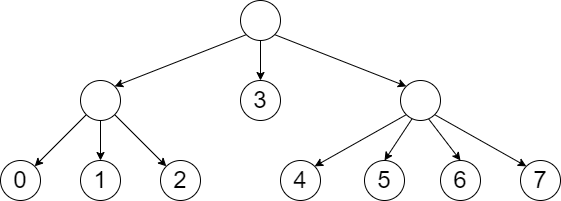
\includegraphics[width=0.7\textwidth]{figure/tree.png} %插入图片,[]中设置图片大小,{}中是图片文件名
\caption{Ternary Search Tree} %最终文档中希望显示的图片标题
\label{fig:tree} %用于文内引用的标签
\end{figure}
\subsubsection{Code}

The code of \verb|pipe-full.hcl| is the same as part B and is omitted here. The core code of \verb|ncopy.ys| is shown in Code Listing \ref{cd:ncopy}.

\begin{lstlisting}[caption={Core Code of ncopy.ys}, label={cd:ncopy}]
# You can modify this portion
	# Loop header
	xorl %eax,%eax		# count = 0;
	iaddl $-8, %edx		# len = len - 8;
	andl %edx,%edx		# len < 0?
	jl Remain		# if so, goto Remain:

Loop:	mrmovl (%ebx), %esi	# read val from src
	mrmovl 4(%ebx), %edi	# read next val from src
	rmmovl %esi, (%ecx)	# store val to dst
	andl %esi, %esi		# val <= 0?
	jle LNpos1		# if so, goto LNpos1:
	iaddl $1, %eax		# count++

LNpos1: rmmovl %edi, 4(%ecx)	# store val to dst
	andl %edi, %edi		# val <= 0?
	jle LNpos2		# if so, goto LNpos2:
	iaddl $1, %eax		# count++

LNpos2: mrmovl 8(%ebx), %esi	# read val from src
	mrmovl 12(%ebx), %edi	# read next val from src
	rmmovl %esi, 8(%ecx)	# store val to dst
	andl %esi, %esi		# val <= 0?
	jle LNpos3		# if so, goto LNpos3:
	iaddl $1, %eax		# count++

LNpos3: rmmovl %edi, 12(%ecx)	# store val to dst
	andl %edi, %edi		# val <= 0?
	jle LNpos4		# if so, goto LNpos4:
	iaddl $1, %eax		# count++

LNpos4:	mrmovl 16(%ebx), %esi	# read val from src
	mrmovl 20(%ebx), %edi	# read next val from src
	rmmovl %esi, 16(%ecx)	# store val to dst
	andl %esi, %esi		# val <= 0?
	jle LNpos5		# if so, goto LNpos5:
	iaddl $1, %eax		# count++

LNpos5: rmmovl %edi,20(%ecx)	# store val to dst
	andl %edi, %edi		# val <= 0?
	jle LNpos6		# if so, goto LNpos6:
	iaddl $1, %eax		# count++

LNpos6: mrmovl 24(%ebx), %esi	# read val from src
	mrmovl 28(%ebx), %edi	# read next val from src
	rmmovl %esi, 24(%ecx)	# store val to dst
	andl %esi, %esi		# val <= 0?
	jle LNpos7		# if so, goto LNpos7:
	iaddl $1, %eax		# count++

LNpos7: rmmovl %edi, 28(%ecx)	# store val to dst
	andl %edi, %edi		# val <= 0?
	jle Next		# if so, goto Next:
	iaddl $1, %eax		# count++

Next:	iaddl $-8, %edx		# len-=8
	iaddl $32, %ebx		# src+=8
	iaddl $32, %ecx		# dst+=8
	andl %edx,%edx		# len >= 0? 
	jge Loop		# if so, goto Loop:

# Maybe just remain less than 8
Remain:	iaddl $5, %edx		# len += 8
	jl Left			# if len < 0, goto Left:
	jg Right		# if len > 0, goto Right:
	je R3			# if len = 0, goto R3:

Left:	iaddl $1, %edx		# len++
	je R2			# if len = 0, goto R2:
	iaddl $1, %edx		# len++
	je R1			# if len = 0, goto R1:
	jmp Done		# goto Done:

Right:	iaddl $-2, %edx		# len -= 2
	je R5			# if len = 0, goto R5:
	jl R4			# if len < 0, goto R4:
	iaddl $-2, %edx		# len -= 2
	je R7			# if len = 0, goto R7:
	jmp R6			# goto R6:

R7:	mrmovl 24(%ebx), %esi	# read val7 from src
	andl %esi, %esi		# val7 <= 0?
	rmmovl %esi, 24(%ecx)	# store val7 to dst

R6:	mrmovl 20(%ebx), %esi	# read val6 from src
	jle R61			# if val7 <= 0, goto R61:
	iaddl $1, %eax		# count++

R61:	rmmovl %esi, 20(%ecx)	# store val6 to dst
	andl %esi, %esi		# val6 <= 0?

R5:	mrmovl 16(%ebx), %esi	# read val5 from src
	jle R51			# if val6 <= 0, goto R51:
	iaddl $1, %eax		# count++

R51:	rmmovl %esi, 16(%ecx)	# store val5 to dst
	andl %esi, %esi		# val5 <= 0?

R4:	mrmovl 12(%ebx), %esi	# read val4 from src
	jle R41			# if val5 <= 0, goto R41:
	iaddl $1, %eax		# count++
	
R41:	rmmovl %esi, 12(%ecx)	# store val4 to dst
	andl %esi, %esi		# val4 <= 0?

R3:	mrmovl 8(%ebx), %esi	# read val3 from src
	jle R31			# if val4 <= 0, goto R31:
	iaddl $1, %eax		# count++

R31:	rmmovl %esi, 8(%ecx)	# store val3 to dst
	andl %esi, %esi		# val3 <= 0?

R2:	mrmovl 4(%ebx), %esi	# read val2 from src
	jle R21			# if val3 <= 0, goto R21:
	iaddl $1, %eax		# count++

R21:	rmmovl %esi, 4(%ecx)	# store val2 to dst
	andl %esi, %esi		# val2 <= 0?

R1:	mrmovl (%ebx), %esi	# read val1 from src
	jle R11			# if val2 <= 0, goto R11
	iaddl $1, %eax		# count++

R11:	rmmovl %esi, (%ecx)	# store val1 to dst
	andl %esi, %esi		# val <= 0?
	jle Done		# if so, goto Done:
	iaddl $1, %eax		# count++

\end{lstlisting}

\subsubsection{Evaluation}

Figure \ref{fig:correctness} shows the correctness of the code. Figure \ref{fig:benchmark} shows that the average CPE is 9.09 and the score is 60.0, which indicates that the code performance is good.

\begin{figure}[htbp] %H为当前位置,!htb为忽略美学标准,htbp为浮动图形
\centering %图片居中
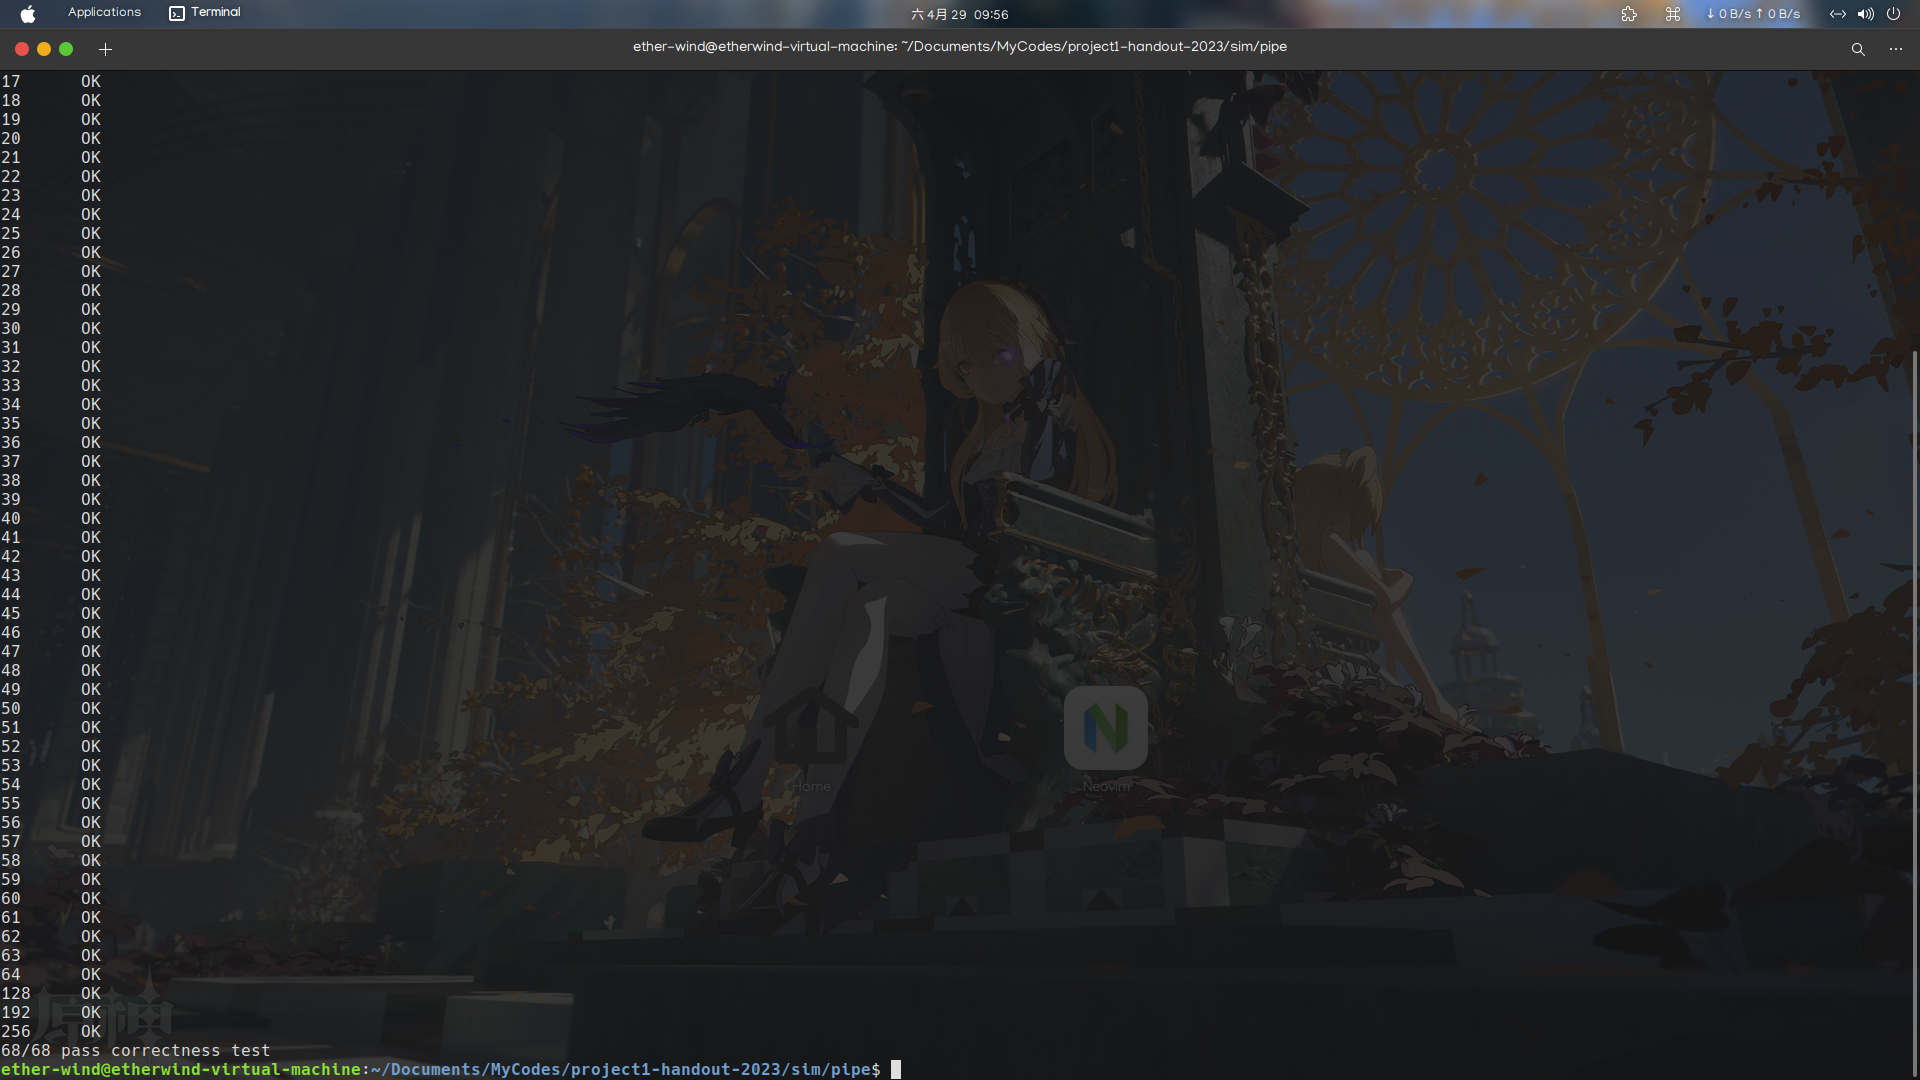
\includegraphics[width=0.9\textwidth]{figure/PartC1.png} %插入图片,[]中设置图片大小,{}中是图片文件名
\caption{Correctness} %最终文档中希望显示的图片标题
\label{fig:correctness} %用于文内引用的标签
\end{figure}

\begin{figure}[htbp] %H为当前位置,!htb为忽略美学标准,htbp为浮动图形
\centering %图片居中
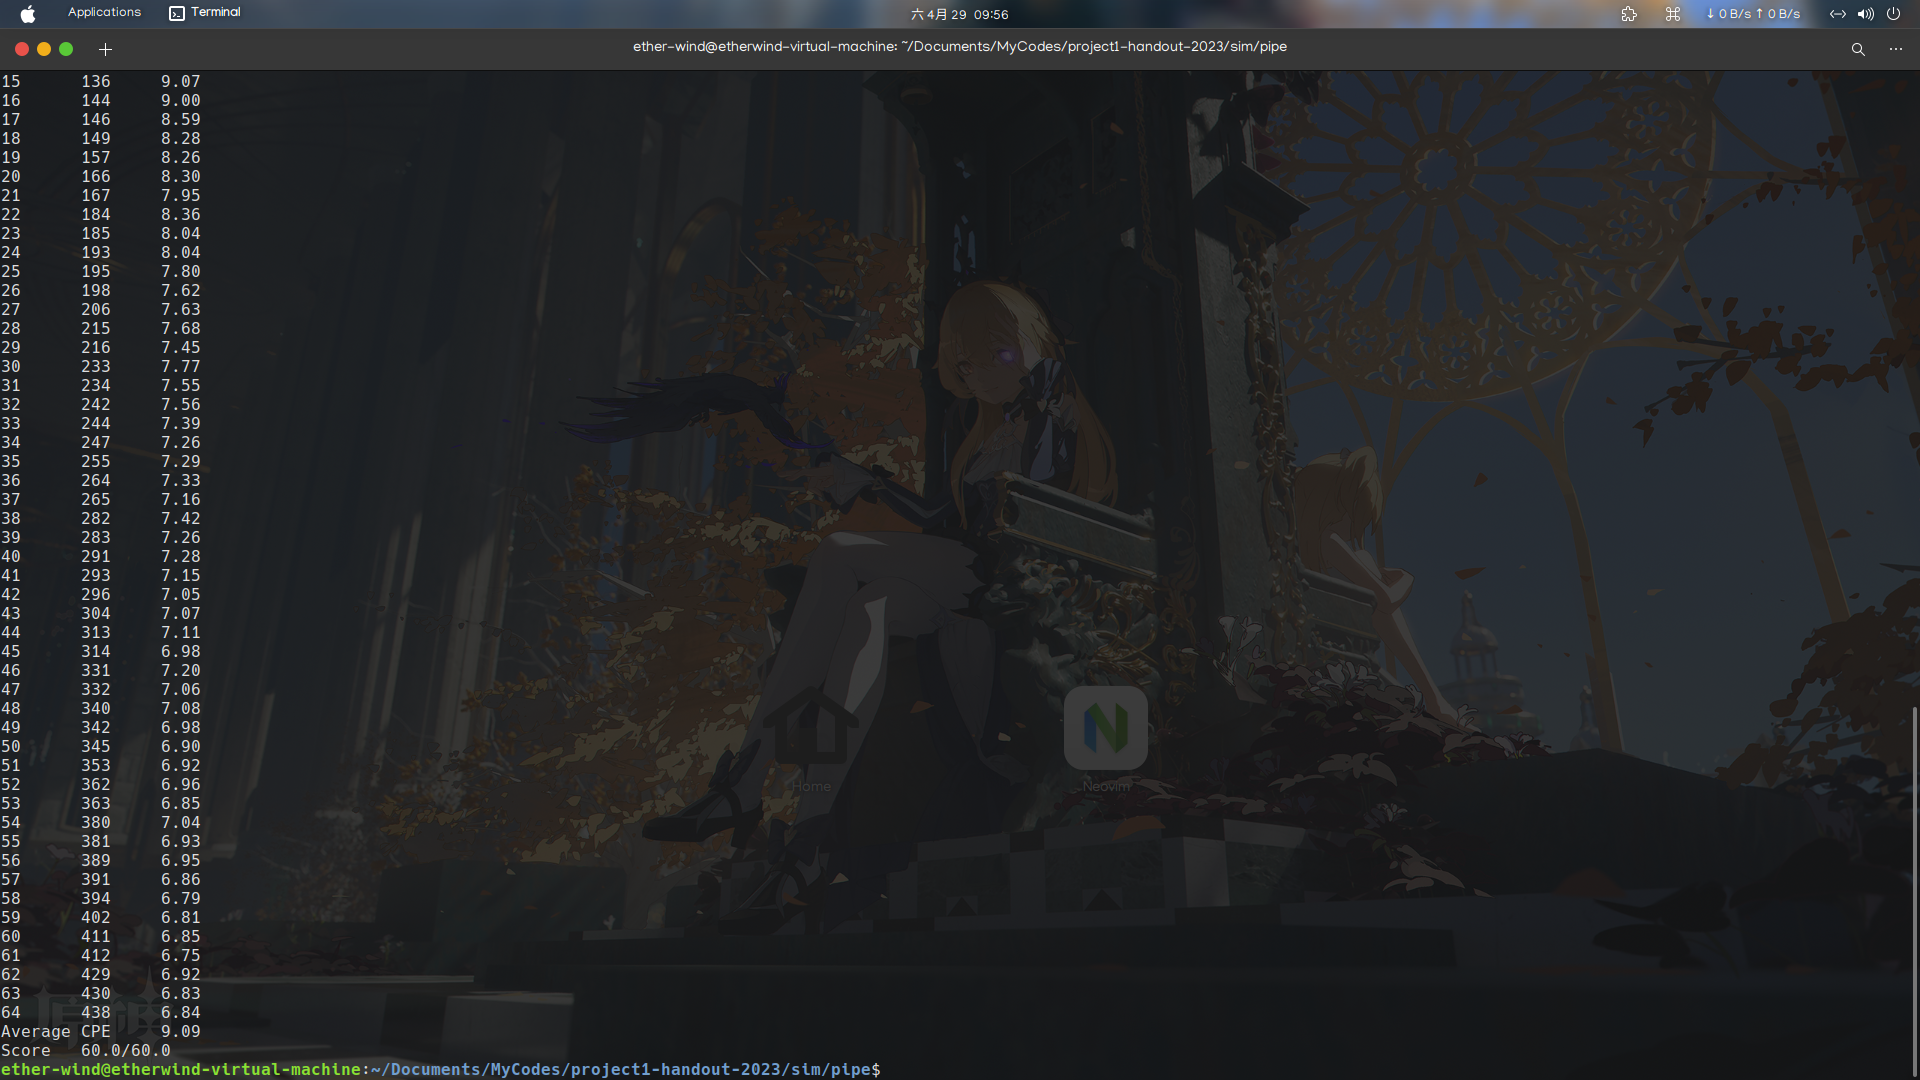
\includegraphics[width=0.9\textwidth]{figure/PartC2.png} %插入图片,[]中设置图片大小,{}中是图片文件名
\caption{Benchmark} %最终文档中希望显示的图片标题
\label{fig:benchmark} %用于文内引用的标签
\end{figure}

\section{Conclusion}

\subsection{Problems}

We encountered the obstacles of understanding and using the Y86 tools, but we compared it to the X86 instructions and finally got a comprehension of it. We faced the trouble of using Linux and running the codes on virtual machine but learned to do it. We found it difficult to optimize the pipeline, but by reviewing the lectures of Computer Architecture we got it done perfectly.

\subsection{Achievements}

In Part C, we adjust code order to avoid data hazards and use several techniques, such as loop unrolling and ternary search tree, to improve the performance of the code. The final average CPE is 9.09, which is a nice performance.

We made adequate annotation in the code part, which greatly enhanced the coding readability. Through the team cooperation, we collaborated smoothly and things did work out. 

%----------------------------------------------------------------------------------------


\end{document}